\documentclass{sigchi}

% Use this section to set the ACM copyright statement (e.g. for
% preprints).  Consult the conference website for the camera-ready
% copyright statement.

% Copyright
\CopyrightYear{2016}
%\setcopyright{acmcopyright}
\setcopyright{acmlicensed}
%\setcopyright{rightsretained}
%\setcopyright{usgov}
%\setcopyright{usgovmixed}
%\setcopyright{cagov}
%\setcopyright{cagovmixed}
% DOI
\doi{http://dx.doi.org/10.475/123_4}
% ISBN
\isbn{123-4567-24-567/08/06}
%Conference
\conferenceinfo{CHI'16,}{May 07--12, 2016, San Jose, CA, USA}
%Price
\acmPrice{\$15.00}

% Use this command to override the default ACM copyright statement
% (e.g. for preprints).  Consult the conference website for the
% camera-ready copyright statement.

%% HOW TO OVERRIDE THE DEFAULT COPYRIGHT STRIP --
%% Please note you need to make sure the copy for your specific
%% license is used here!
% \toappear{
% Permission to make digital or hard copies of all or part of this work
% for personal or classroom use is granted without fee provided that
% copies are not made or distributed for profit or commercial advantage
% and that copies bear this notice and the full citation on the first
% page. Copyrights for components of this work owned by others than ACM
% must be honored. Abstracting with credit is permitted. To copy
% otherwise, or republish, to post on servers or to redistribute to
% lists, requires prior specific permission and/or a fee. Request
% permissions from \href{mailto:Permissions@acm.org}{Permissions@acm.org}. \\
% \emph{CHI '16},  May 07--12, 2016, San Jose, CA, USA \\
% ACM xxx-x-xxxx-xxxx-x/xx/xx\ldots \$15.00 \\
% DOI: \url{http://dx.doi.org/xx.xxxx/xxxxxxx.xxxxxxx}
% }

% Arabic page numbers for submission.  Remove this line to eliminate
% page numbers for the camera ready copy
% \pagenumbering{arabic}

% Load basic packages
\usepackage{balance}       % to better equalize the last page
\usepackage{graphics}      % for EPS, load graphicx instead 
\usepackage[T1]{fontenc}   % for umlauts and other diaeresis
\usepackage{txfonts}
\usepackage{mathptmx}
\usepackage[pdflang={en-US},pdftex]{hyperref}
\usepackage{color}
\usepackage{booktabs}
\usepackage{textcomp}

% Some optional stuff you might like/need.
\usepackage{microtype}        % Improved Tracking and Kerning
% \usepackage[all]{hypcap}    % Fixes bug in hyperref caption linking
\usepackage{ccicons}          % Cite your images correctly!
% \usepackage[utf8]{inputenc} % for a UTF8 editor only

% If you want to use todo notes, marginpars etc. during creation of
% your draft document, you have to enable the "chi_draft" option for
% the document class. To do this, change the very first line to:
% "\documentclass[chi_draft]{sigchi}". You can then place todo notes
% by using the "\todo{...}"  command. Make sure to disable the draft
% option again before submitting your final document.
\usepackage{todonotes}

% Paper metadata (use plain text, for PDF inclusion and later
% re-using, if desired).  Use \emtpyauthor when submitting for review
% so you remain anonymous.
\def\plaintitle{A SYSTEMATIC LITERATURE REVIEW: EFFECT OF CODE SMELLS ON NON-FUNCTIONAL ATTRIBUTES OF SOURCE CODE}
\def\plainauthor{First Author, Second Author, Third Author,
  Fourth Author, Fifth Author, Sixth Author}
\def\emptyauthor{}
\def\plainkeywords{Authors' choice; of terms; separated; by
  semicolons; include commas, within terms only; required.}
\def\plaingeneralterms{Documentation, Standardization}

% llt: Define a global style for URLs, rather that the default one
\makeatletter
\def\url@leostyle{%
  \@ifundefined{selectfont}{
    \def\UrlFont{\sf}
  }{
    \def\UrlFont{\small\bf\ttfamily}
  }}
\makeatother
\urlstyle{leo}

% To make various LaTeX processors do the right thing with page size.
\def\pprw{8.5in}
\def\pprh{11in}
\special{papersize=\pprw,\pprh}
\setlength{\paperwidth}{\pprw}
\setlength{\paperheight}{\pprh}
\setlength{\pdfpagewidth}{\pprw}
\setlength{\pdfpageheight}{\pprh}

% Make sure hyperref comes last of your loaded packages, to give it a
% fighting chance of not being over-written, since its job is to
% redefine many LaTeX commands.
\definecolor{linkColor}{RGB}{6,125,233}
\hypersetup{%
  pdftitle={\plaintitle},
% Use \plainauthor for final version.
%  pdfauthor={\plainauthor},
  pdfauthor={\emptyauthor},
  pdfkeywords={\plainkeywords},
  pdfdisplaydoctitle=true, % For Accessibility
  bookmarksnumbered,
  pdfstartview={FitH},
  colorlinks,
  citecolor=black,
  filecolor=black,
  linkcolor=black,
  urlcolor=linkColor,
  breaklinks=true,
  hypertexnames=false
}

% create a shortcut to typeset table headings
% \newcommand\tabhead[1]{\small\textbf{#1}}

% End of preamble. Here it comes the document.
\begin{document}

\title{\plaintitle}

\numberofauthors{3}
\author{%
  \alignauthor{Nazira Munalbayeva\\
    \affaddr{University of Salerno}\\
    \affaddr{Salerno, Italy}\\
    \email{n.munalbayeva@studenti.unisa.it}}\\

}

\maketitle

\begin{abstract}
  \textit{Context}: Code smells adversely effect on software quality and impede its maintenance and development. Therefore, in recent years, in the software community, this topic has become relevant for research. \\
  \textit{Objective}: The main goal of this work is to study current researches and determine the relationship between smells and non-functional attributes.\\
  \textit{Method}: We had an overview about code smells effect on non-functional attributes, and what tools and techniques have been used to study this relationship. We studied 21 primary studies in detail and synthesized results.\\ 
  \textit{Results}: Maintainability, performance, and security are more affected by code smells. The code smells that most affect different quality non-functional attributes are GodClass, LongMethod, SpaghettiCode and FeatureEnvy. GodClass. 
  
  
\end{abstract}

\keywords{\textit{Systematic Review, Secondary Studies, Code smells, Anti-patterns, Non-functional attributes, Non-functional requirements}}

\section{Introduction}

Non-functional requirements (NFR) are recognized as very important factors for software projects \cite{Chung}, \cite{Firesmith}, \cite{Ebert}. If the NFRs are not properly resolved, a number of potential problems may arise. For example, software may be of poor quality, or developers may spend more time and money to fix software errors \cite{Chung}. One reason for poor quality is code smells. Code smells refers to an anomaly in the source code that demonstrates a violation of basic design principles, such as encapsulation, modularity, abstraction, and hierarchy \cite{Booch}. They appear in poor design and poor implementation methods. Code smells are the main reasons indicating possible flaws in the development of a software system. \cite{Fowler}. There are many types of code smells that can affect a class, a separate method, their group, or an entire subsystem. Also, they can impact on non-functional requirements, such as testability \cite{Sabane}, maintainability \cite{Yamashita} \cite{Palomba}, comprehensibility \cite{Abbes}, performance, reliability \cite{Jaafar} and etc.
In recent years, code smells have been studied for various reasons. The main reason is the negative impact on software quality. Software quality is an important aspect, therefore there is a large number of research works in this area. A large number of scientific papers require analysis and synthesis. Analyzing and synthesizing available information can help the software community understand existing knowledge and identify problems.
There have been a few attempts to understand current practices and provide an overview of the existing knowledge about software smells. Singh et al. \cite{Singh} provide a systematic literature review (SLR) on code smells and refactoring in object-oriented software systems. The review covers 238 primary studies. The study focuses on methods and tools for detecting code smells. Also in this review, methods and tools for their refactoring were analyzed. 
Similarly, Zhang et al. \cite{Zhang} reviewed the studies from 2000 to 2009. They find such gaps in the literature: modern studies choose a small amount of smells for their research, some smells are poorly studied by the community, such as message chains. In addition, the study emphasizes that the effects of code smells are poorly understood.
Therefore, Cairo et al. \cite{Cairo} reviewed the impact of code smells on Software Bugs. The review consisted of references over the past decade to this topic. Based on the results of the research was discovered the influence of code smells on the appearance of various software bugs.
Also, Sharma et al. \cite{Sharma} investigated smell-related resources published between 1999 and 2016. They presented the available knowledge in a generalized form. They classified detection methods of smell. The authors concluded that currently available tools can detect only a very small amount of smells.
After reviewing many articles, we noticed that there was no systematic review of the effect of code smells on NFAs. Therefore, we began to conduct this SLR to reduce research gaps. In this study, we examine the effects of code smells on NFAs of source code.  Our goal is to identify and analyze how code smells affect to NFAs.
The rest of the article is organized as follows: Section 2 - presents the research methodology. Section 3 - provides answers to research questions. Section 4 - Threats to validity, Section 5 - outlines the limitations of this work, and section 6 - outlines the conclusions of the systematic review.


\section{Research Metodology}
We planned, conducted, and reported the review by following the SLR process suggested by Kitchenham et all. \cite{Kitchenham}. The protocol for this review was developed during the planning phase of this SLR. The protocol includes six stages: research questions, search strategy design, study selection, quality assessment, data extraction, and data synthesis. After the formation of the review protocol, a number of steps were taken in the review. At the first stage, we formed research questions that must be answered in the SLR. In the second step, we described a search strategy, including the search terms and the selection of sources to identify primary research. The third step is to identify relevant studies based on research questions. This step also defines the inclusion and exclusion criteria for each primary study. At the next stage, we determine the criteria for assessing quality by creating a quality assessment questionnaire for analysis and evaluation of studies. The final steps involve the data extraction process to collect the necessary information to answer research questions, and we also in this step develop methods for data synthesis. In the following Subsection we will present the details of the process. 

\begin{figure}[h]
\centering
  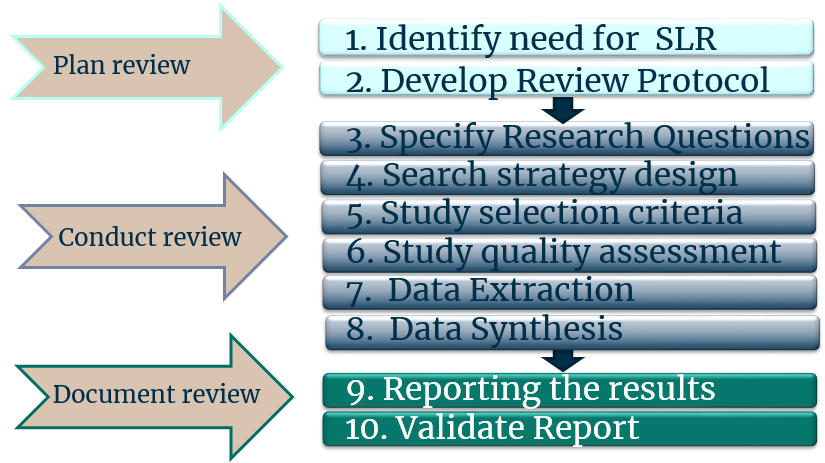
\includegraphics[width=1\columnwidth]{Figures/1}
  \caption{Systematic literature review process.}~\label{fig:figure1}
\end{figure}

\subsection{Research questions}
With this project, we want to investigate how much code smells impact on a system, and which are their effects on non-functional requirements. In order to achieve our goal, we will analyze many scientific researches and try to answer our questions. The main goal of this work is to study current research and determine the relationship between smells and NFAs. To structure our studies and RQs we studied and evaluated other tertiary studies \cite{Imtiaz},\cite{Khan}, that helped to understand how to constructed RQs. 
We aim to answer the following research questions by conducting the SLR: \\
\textbf{RQ1:} In which way a Code Smell Impact on NFAs? \\
\textbf{RQ2:} How the connection between code smells and NFAs was determined? \\
\textbf{RQ3:} Are all code smells impactful on NFAs? 

\subsection{Search strategy and study selection}

The search involved in four digital libraries: IEEEXplore, ACM, Elsevier, and Scopus. The syntax of the search string was the same for all libraries, including only the title, keywords, and abstract. Only for searching in Scopus we a little bit changed and adapted the search string. We formed the search string by incorporating alternative terms and synonyms using boolean expression ‘OR’ and combining main search terms using ‘AND’. The following general search string were used for the identification of primary studies: ("Non-functional attributes" OR "NFA" OR "Non-functional requirements") AND ("code-smell" OR "bad smell" OR "code anomalies") AND ("effect" OR "impact" OR "influence") (“Anti patterns” OR “APs” OR “Anti-pattern”). We also added anti-patterns in search terms, because software engineering researchers and practitioners often use the terms “anti-pattern” and “smell” interchangeably [18]. 
We started the review with an automatic search, supplemented by a snowballing process, to identify potentially important studies. The snowball entailed following links from one article to another to find other related articles \cite{Skoglund}. This was done both in the opposite and in the forward direction. The snowballing in the opposite direction means following the list of references, and the forward direction means referring to papers concerning an article that was deemed relevant. Potentially relevant studies were identified based on an analysis of their names and annotations. Immediately discarded studies that were not related to the search. Duplicate reports were removed during the selection process.
The identified articles were assessed to determine if they met the following screening criteria. The inclusion and exclusion criteria are shown in Table-1. \\

\begin{table}[h]
	\small
	\begin{tabular}{ p{35mm} |  p{35mm}}
		\toprule
		\textbf{Inclusion Criteria} & \textbf{Exclusion Criteria}\\
		\midrule
		1. The article should be published in a scientific journal or conference; & 1. Publications published before 2010;\\
		2. Publications published from 2010 January; & 2.	Research-based solely on expert advice, without convincing evidence;\\
		3. Publications that involve an empirical study; & 3. Studies that are focused only on code smells or on NFA of source code without any discussion regarding the relationship and/or influence that the first exert on the second;\\
		4. If several journal articles report the same study, the most recent article should be included. & If several journal articles report the same study, the last study should be excluded. \\
		\bottomrule
	\end{tabular}
	\caption{Inclusion and Exclusion criteria}~\label{tab:in_ex_criteria}
\end{table}

\subsection{Quality assessment criteria}
We formed a questionnaire to assess the relevance and quality of research. The quality questionnaire was developed taking into account proposals submitted by Kitchenham et al. \cite{Kitchenham}. In the Table-2 presents the quality assessment questions that were used to weight the studies. All artifacts obtained as a result of the study selection process are available in the GitHub repository \cite{Munalbayeva}. 

\begin{table}[h]
	\small
	\begin{tabular}{ p{5mm} |  p{65mm} | p{3mm} | p{3mm}}
		\toprule
		\textbf{Q \#} & \textbf{Quality questions} & \textbf{Yes} & \textbf{No}\\
		\midrule
		Q1 & Is there a clear statement of the research objectives?  & & \\
		Q2 & Is the document based on empirical evidence?  & & \\
		Q3 & Are the estimation methods well defined and deliberate? & & \\
		Q4 & Are methods and tools for determining the effects of code smells described? & & \\
		Q5 & Have certain types of code smells been analyzed? & & \\
		Q6 & Have types of NFAs been analyzed?& & \\
		Q7 & Are the effects of code smells on the NFA determined?& & \\
		Q8 & Are the limitations of study analyzed explicitly?& & \\
		\bottomrule
	\end{tabular}
	\caption{Quality assessment questions.}~\label{tab:assess_criteria}
\end{table}

Only those research papers that can answer all quality assessment questions positively were included in the SLR. Finally, after careful reviews, discussions, and brainstorming sessions, the final decision on inclusion / exclusion for each study was made. All stages and results of study selection process are shown in the Figure 2 and in repository \cite{Munalbayeva}.


\begin{figure}[h]
	\centering
	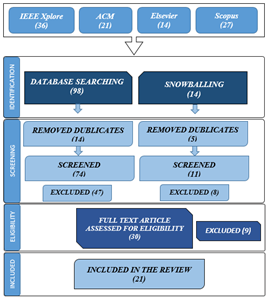
\includegraphics[width=1\columnwidth]{Figures/2}
	\caption{Study selection process.}~\label{fig:figure1}
\end{figure}

\subsection{Data extraction and data synthesis}
Based on the results of the selection process described previously, we listed and classified the selected primary studies to enable a clear understanding of aims, methodologies, and findings. We structured the spreadsheet for data extraction. In this form, we find the main information that we consider relevant regarding the papers \cite{Munalbayeva}. In general, we consider:\\
\textbf{1.}	identification number; \\
\textbf{2.}	year; \\
\textbf{3.}	title; \\
\textbf{4.}	objectives or aims;\\ 
\textbf{5.}	code smells; \\
\textbf{6.}	analysed projects;\\
\textbf{7.}	research questions and respective answers;\\
\textbf{8.}	In which way a Code Smell Impact on NFAs? \\
\textbf{9.}	How the connection between code smells and NFAs was determined? \\
\textbf{10.} Are all code smells impactful on NFAs? \\

The basic objective while synthesizing data is to accumulate and combine facts and figures from the selected primary studies in order to formulate a response and resolve the research questions. Collection of a number of studies which state similar and comparable viewpoints and results helps in providing research evidence for obtaining conclusive answers to the research questions.  We utilize a number of techniques to synthesize data collected from our primary studies. In order to answer the research questions, we used visualization techniques such as line graph, box plots, pie charts and bar charts. We also used tables for summarizing and presenting the results. 

\section{Discussion and Result}
This section presents and discusses the findings of this review. Firstly, we present an overview of the selected studies. It also outlines the characteristics of the selected studies which are listed in Table A in the Appendix. Studies are indicated by the letter "S" and the corresponding number. Table A in the Appendix provides a unique identifier for each selected primary study along with a link. These identifiers will be used in all subsequent sections to refer to their primary research. Secondly, we report and discuss the review findings according to the research questions, one by one in the separate subsections. 

\subsection{Overview of selected studies}

We identified 21 studies (see Table 6 in Appendix) in the field of effects of code smells on NFA. These papers were published during the time period 2010-2020. Among them, 14 (66\%) papers appeared in conference proceedings, 6 (34\%) papers were published in journals. 
Figure 3 depicts the time distribution of the selected studies. 

\begin{figure}[h]
	\centering
	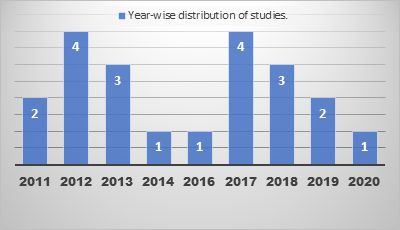
\includegraphics[width=1\columnwidth]{Figures/3}
	\caption{Timeline distribution of papers.}~\label{fig:figure1}
\end{figure}

In this SLR we researched the NFAs as maintainability, reliability, performance, and security. The pie chart (Figure 4) describes the percentage of attributes that are included in the SLR. We can see that maintainability has received dominant attention in recent years and 50\% of the literature included in the review about the effect of code smells on maintainability. 

\begin{figure}[h]
	\centering
	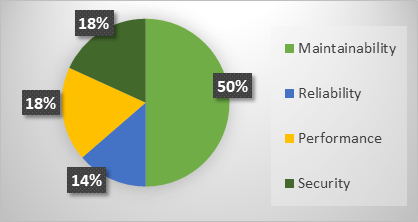
\includegraphics[width=1\columnwidth]{Figures/4}
	\caption{Percentage of included attributes in the review \%.}~\label{fig:figure1}
\end{figure}

Further in Table-3 we can see the list of active authors, that researching the influence of code smells on different non-functional attributes. The second column of the table indicates their articles that were included in this SLR.

\begin{table}[h]
	\small
	\begin{tabular}{ p{5mm} |  p{30mm} | p{30mm}}
		\toprule
		\textbf{N} & \textbf{Authors} & \textbf{Numbers of Study} \\
		\midrule
		1 & Aiko Yamashita  &  S6, S9 \\
		2 & Fabio Palomba  & S17, S20  \\
		3 & Foutse Khomh & S1, S4, S5, S8, S21 \\
		4 & Gabriele Bavota & S3, S17 \\
		5 & Giuliano Antoniol &S1, S4, S7  \\
		6 & Massimiliano Di Penta& S4, S7, S17 \\
		7 & Pascal Gadient & S13, S16 \\
		8 & Yann-Gaël Guéhéneuca& S1, S4, S7, S8, S21 \\
		\bottomrule
	\end{tabular}
	\caption{Active authors that researching relationships between NFAs and code smells.}~\label{tab:assess_criteria}
\end{table}


Figure-5 describes how many research papers have studied code smells that impact on non-functional attributes. We found that GodClass was investigated in 13 articles and is the most relevant smell of codes that impacts too many types of NFAs. Also, SpaghettiCode, MessageChain, RefusedBequest, and FeatureEnvy was explored in 6-8 articles in this SLR.  

\begin{figure}[h]
	\centering
	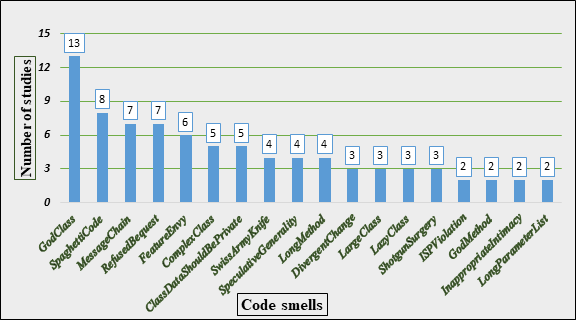
\includegraphics[width=1\columnwidth]{Figures/5}
	\caption{Number of articles that studied code smells impact.}~\label{fig:figure1}
\end{figure}

\subsection{RQ1: In which way a Code Smell Impact on NFA?}

In this subsection, we use evidence collected from the selected studies to answer Research Question (RQ1): In which way a Code Smell Impact on NFA? In the Table-3 presents how each of the selected studies contributed to answer RQ1. In this case, the following 21 studies provide evidence of the influence code smells on NFA. We divided them into groups, in connection with the attributes that were investigated in them.

\begin{table}[h]
	\small
	\begin{tabular}{ p{20mm} |  p{50mm}}
		\toprule
		\textbf{NFAs} & \textbf{Study}\\
		\midrule
		Maintainability & S1, S2, S3, S4, S5, S6, S7, S9, S15, S17, S21\\
		Reliability  & S4, S8, S10\\
	Performance & S11, S14, S18, S20\\
		Security & S12, S13, S16, S19 \\
		\bottomrule
	\end{tabular}
	\caption{Attributes and studies. }~\label{tab:in_ex_criteria}
\end{table}

\subsubsection{Mantainability}
One important non-functional attribute is maintainability. Recently, many scientists have begun to figure out the effect of code smells on maintainability. Code smells indicate problems with code quality, such as comprehensibility and variability, which can lead to faults. Also, the presence of code smells decreases the understandability of the code and leads to an increase in the cost of maintenance. To help reduce the cost of maintenance, the researchers proposed several approaches that make it easier to understand the program and identify parts of the source code of software systems that are prone to changes and faults. Further, take a closer look at how code smells effect on maintainability. 

Abbes et al. \cite{Abbes} determined that systems with combinations of anti-patterns as Blob and Spaghetti code take longer to understand. They require more effort and force subjects to respond less correctly. Understanding the code was easy when the system did not contain any anti-patterns. The results Bavota et al. \cite{Bavota} show that smells of test code are quite common in software systems and that they adversely affect the maintainability of software systems. More precisely, they affect the accuracy and time of test suites. Sjoberg et al. \cite{Sjoberg}, found that files with Feature Envy and God Class code smells are used for several purposes, and the implementation is used instead of the interface. Shotgun Surgery was associated with more effort than files without these smells. The smell of Refused Bequest was associated with a slight decrease in effort. Also, Politowski et al, \cite{Politowskia}, defined that the anti-pattern Blob or Spaghetti Code present in the source code reduces the productivity of developers, increasing the time spent on tasks, reducing the accuracy of their answers and increasing their necessary efforts. Romano et al. \cite{Romano}, analyzed that Classes affected by anti-patterns change more often as the system develops. Classes affected by antipatterns Complex Class, Spaghetti Code, and SwissArmyKnife are more likely to change than classes affected by other antipatterns. Certain antipatterns lead to certain types of source code changes, for example, API changes appear more often in classes affected by Complex Class, Spaghetti Code and SwissArmyKnife antipatterns. Zazworka et al. \cite{Zazworka} show that the god classes are generally more prone to change, and in some cases more prone to defects. This is a strong indicator that the smell of the god class is important for monitoring and management in software development projects, and that they are actually associated with technical debt. Also, Palomba et al. \cite{Palomba2}, determined, that classes that are affected by code smells have a statistically significant higher change and fault susceptibility than classes that are not affected by code smells. In addition, the authors observed a very clear trend, indicating that the higher the number of smells affecting the class, the higher its change- and fault-proneness. Yamashitaa et al. \cite{Yamashita}, concluded that systems that contain more code smells than others are too complex and comprehensive. These systems will be very difficult to maintain. They affect to maintainability factors: Design suited to problem domain, Inheritance, Simplicity, Use of components, Design consistency, Logic Spread.
Ban et al. \cite{Ban}, demonstrated that anti-patterns adversely affect the maintainability of software. The most important ones to avoid are Long Functions, Large Class Codes and Shotgun Surgeries. As for the Shotgun Surgery, the main goal is to reduce the connection by moving or retrieving methods or fields, or even identifying a superclass.
Considering all the above results, we can conclude that almost all the smells of the code affect the maintainability of the system. But as shown in studies, different smells affect differently, the authors advise paying attention to smells that complicate understanding of the code. Accordingly, which require more time and effort. Effect of code smells to maintainability shown in the Table-4. We can see that God Class and Spaghetti Code more impacts to maintainability quality.

\begin{table}[h]
	\small
	\begin{tabular}{ p{35mm} |  p{45mm}}
		\toprule
		\textbf{Quality aspects} & \textbf{Code smells}\\
		\midrule
		Simplicity and comprehension & GodClass, GodMethod, LazyClass, MessageChains, LongParameterList, SpaghettiCode\\
		Design consistency  & AlternativeClasseswithDifferentInterfaces, ISPViolation, DivergentChange, TemporaryField\\
		Time – consuming & SpaghettiCode, GodClass\\
		Effort – consuming & ShotgunSurgery, SpaghettiCode, GodClass \\
		Change – prone & InappropriateIntimacy, LongMethod, SpaghettiCode, SpeculativeGenerality, ComplexClass, RefusedBequest, SwissArmyKnife, GodClass \\
		Require a higher number of test cases & GodClass, ComplexClass, AntiSingleton, SwissArmyKnife \\
		Increase future maintenance costs & GodClass \\
		\bottomrule
	\end{tabular}
	\caption{Code smells impact to maintainability }~\label{tab:in_ex_criteria}
\end{table}

\subsubsection{Reliability}
Software reliability is the likelihood that a program runs smoothly for a period of time. Malfunctions in the system during operation occur due to faults. Sometimes code smells are the cause of such failures. They negatively affect systems, making classes more fault-prone. 
Khomh  et al. \cite{Khomh} determined that classes with anti-patterns are more likely to be subject to high fault-fixing changes. Specifically, they found the Message Chain is consistently associated with a high fault rate. Jaafar et al. \cite{Jaafar} observed three systems (ArgoUML, JFreeChart, and XercesJ) with 12 types of anti-patterns and their dependencies on faults. They concluded that if classes changed with anti-patterns, they will be significantly more fault-prone than other similar classes. However, they do not rule out the possibility that there will be no impact on fault tolerance for classes that have been modified with SpaghettiCode, ClassDataShouldBePrivate, ComplexClass, and LongParameterList. Also, Hall et al \cite{Hall}, investigated the relationship between faults and code smells in three systems, such as Eclipse, ArgoUML, and Apache Commons. In different systems, code smells affected the appearance of faults in the system in different ways. For example, there is a significant relationship between failures and MessageChains in two systems. In cases where DataClumps is combined with large files, there are more crashes in two systems, and less in one. On two systems containing MessageChains, they are associated with a large number of errors. These results show that code smells manifest themselves differently in different systems, probably depending on the application area and development context.

\subsubsection{Performance}

Performance determines how well a system performs certain functions under certain conditions. Examples are response speed, bandwidth, power consumption, and storage capacity. Service levels, including performance requirements, are often based on end-user support. Therefore, the studies included in the SLR are mainly related to the Android system. Hecht et al. \cite{Hecht}, provides that the code smells Getter / Setter (IGS), MemberIgnoringMethod (MIM), and HashMapUsage (HMU) have a significant impact on the user interface and memory performance. Correcting these smells in the Android code effectively improves the user interface and memory performance. Carette et al. \cite{Carette} found that fix at least one smell of Android code (HMU, IGS or MIM) reduces the power consumption of the mobile phone. Verdecchia et al. \cite{Verdecchia} proved that refactoring code smells can lead to a significant reduction in power consumption of software applications. Refactoring code smells positively affects the environmental aspect by reducing the energy impact of software and the technical aspect by increasing the convenience of maintaining software over time. Also, Palomba et al. \cite{Palomba3} investigate the Impact of Code Smells on the Energy Consumption of Mobile Applications. Code smells such as InternalSetter, LeakingThread, MemberIgnoringMethod and SlowLoop consume 87 times more than methods that are affected by other code smells. Moreover, the authors found that refactoring these code smells reduces energy consumption in all situations. 

\subsubsection{Security}

Software security is one of the most pressing issues in Software Engineering. Therefore, vulnerabilities that are manifested due to code smells have been studied. For instance, Islam et al. \cite{Islam} found that security vulnerabilities in cloned code are significantly more dangerous than in non-cloned code. Clones are syntactically identical code fragments with variations in identifier names, literals, types, layout and comments, and also allow further differences, such as adding, deleting, or modifying operators that are most unsafe. 
Ghafari et al. \cite{Ghafari} investigated 160 applications and found that despite the variety of applications in terms of popularity, size, and release date, most suffer from at least three different smells of security. And the smells of security are actually an indicator of security vulnerabilities.
Gadient ae al. \cite{Gadient} found that the default value for task affinity configurations does not protect the application from theft of user interface components. A system that contains code smells like DenialofService, IntentSpoofing, IntentHijacking is more vulnerable than a system that does not contain this code smells.
Elkhail et al. \cite{Elkhail} discovered that code smells can slow down the development process and can increase the risk of faults and crashes. 

\textbf{Summary for RQ1}\\
Maintainability, performance, and security are more affected by code smells. The code smells that most affect different quality non-functional attributes are GodClass, LongMethod, SpaghettiCode and FeatureEnvy. GodClass most affects attribute quality. This affects maintainability, complexity, changeability, and performance. Feature Envy and InappropriateIntimacy make the code more change-prone. ComplexClass, SpaghettiCode, and SwissArmyKnife make the code more change-prone. If the source code contains a combination of code smells, it most reduces the quality of non-functional attributes. Therefore, a combination of all kinds of code smells should be avoided. To prevent the impact of code smells on performance, we basically need to refactor the code. Code smells of the Android system, e. g. Getter / Setter (IGS), MemberIgnoringMethod (MIM), and HashMapUsage (HMU) mostly affect performance aspects like user interface, Energy Consumption, and memory performance. Code smells on security can slow down the development process and can increase the risk of faults and crashes. Thus, it will increase the risks of software security vulnerabilities. The most impactful code smells on security is DenialofService, IntentSpoofing, IntentHijacking.

\subsection{RQ2: How the connection between code smells and NFA was determined? }

To answer this question, we scanned all articles that were included in the systematic analysis. Defined that different tools and techniques were used to determine the relationship between code smells and NFAs. Depending on the NFAs, this process was carried out differently. But  articles in this SLR extensively used the DECOR method (Detection of dEfects for CORrection) to detect code smells [\cite{Abbes}, \cite{Khomh}, \cite{Romano}, \cite{Romano}, \cite{Jaafar}, \cite{Politowskia}]. Abbes et al. \cite{Abbes} conducted an Empirical Study of the Impact of anti-patterns On Program Comprehension. They used the Detex anti-pattern detection technique, which is based on the DECOR method, to ensure that every system has at least one occurrence of the Blob anti-pattern or SpaghettiCode. Then authors confirm the classes manually. For the experiment, they used a combination of one Blob and one SpaghettiCode to analyze its effects on understandability of source code. Then they measured the effort and the subjective workload of the task using the NASA Task Load Index (TLX). Later, Politowskia et al. \cite{Politowskia} continued this experiment. They used different tasks, each participant was assigned 2 systems: one containing two occurrences of the Blob anti-pattern or spaghetti code, and one without any anti-pattern. They measured average correct answers, time and effort spend for understanding the impact of anti-patterns. Also, they measured the participant's effort using the NASA Task Load Index. To analyze statistical computing was used the R9 software environment, which consisted of a preliminary analysis and a statistical hypothesis test. For preliminary analysis, the authors applied descriptive statistics to the dependent variables and used boxplots10 to analyze the data. They tested null hypotheses using the linear mixed model analysis method. In most cases, researches used methods for detecting code smells, such as Metrics-based smell detection, History-based smell detection, and Machine learning-based smell detection. In some studies, refactoring code smells has been used effectively to detect the effects of code smells [\cite{Zazworka}, \cite{Sabane}, \cite{Sjoberg}, \cite{Hall}, \cite{Islam}, \cite{Carette}, \cite{Verdecchia}, \cite{Palomba3}]. They compared to code that contained code smells and code after refactoring code smells. Palomba et al. \cite{Palomba3} conducted a research to identify the Impact of Code Smells on Energy Consumption. The authors performed an analysis using the aDoctor and PETrA tools. These tools were developed and evaluated by the authors earlier. aDoctor is an Android-specific code smell detector that extracts structural properties from source code to detect code smells. PETrA is a software tool that evaluates the energy profile of mobile applications. Using these tools, they found that some code smells are causes 87 times more energy consumption than other code smells. In addition, they used the refactoring method as a way to increase energy efficiency by removing the smell of code. As a result, it was known that it was possible to increase the energy efficiency of source code methods by refactoring code smells. 

\subsection{Summary for RQ2.}
To answer the RQ2 we focused on the frequent methods that were used in research papers to determine the effect of code smells on NFAs. There is still no universal method to detect all types of code smells and also, in different systems, code smells differently exert their influence. These factors influenced the creation of different techniques and tools. In several studies, they used the refactoring method to find the connection between code smells and NFAs.   

\subsection{RQ3: Are all code smells impactful on NFA? }
In previous research questions, we determined that code smells affect NFAs in different ways. In response to this question, we wanted to find out whether some code smells might not affect the NFAs, so that the developers would not spend effort on refactoring in some cases. And analyzing the articles included in the SLR, we found that some types of code smells affect the factors of NFAs less. Abbes et al. \cite{Abbes} found that the appearance of one anti-Blob pattern or one spaghetti code in the source code of a software system does not complicate its comprehensibility. Researchers have compared the source code without an anti-pattern to verify this. Bavota et al. \cite{Bavota} investigated the effect of test smells on maintainability. They concluded that the Lazy Test smell does not have a strong effect on program maintenance and comprehension. Sabane et al. \cite{Sabane} determined that classes with anti-patterns like method chains or Lazy Classes do not greatly affect the cost of testing. Sjoberg et al. \cite{Sjoberg} explored the quantitative impact of code smells on maintenance efforts. They found that code smell RefusedBequest was associated with less effort than other code smells.  Hall at al. \cite{Hall} conducted their experiment on different systems like Eclipse, ArgoUML, and Apache Commons and investigated the effect of five smells on the number of faults. The results show that smell SwitchStatements did not affect failures in all three systems. It was also discovered that DataClumps increased the number of Faults in one system, but reduced the number of faults in two other systems. The results show that smells manifest differently in systems, probably depending on the subject area and development context. Researchers also found that certain smells reduce the number of faults rather than increase them. For example, MiddleMan reduced the number of faults in ArgoUML, and SpeculativeGenerality reduced in Eclipse. This is an important conclusion, as it suggests that arbitrary code smells refactoring can actually be unproductive. 

\subsection{Summary for RQ3.}
Analyzing the results, we can conclude that code smells are not always the main cause of errors in the code. Sometimes some types of smells reduce faults. Also refactoring is not an absolute solution to improve the quality of the code.


\section{THREATS TO VALIDITY}

The following validity issues were considered in interpreting the results of this review. In substantiating the conclusion, there is a risk of biased data extraction. This was resolved by defining a form of data mining to answer research questions. Conclusions and implications are based on the extracted data. Threats to internal validity were considered at the review selection stage. The studies included in this review were identified through a rigorous multi-stage selection process. The studies identified in the SLR have been compiled from numerous literature databases covering relevant journals and conferences. One possible threat is bias in the choice of publications. In the present work, this was solved by specifying a research protocol that defines research questions and research objectives, inclusion and exclusion criteria, search strings that will be used in the information search strategy and data extraction strategy. Another potential bias is due to code smells. This makes it possible not to paint the whole picture, because not all code smells and, their effect on NFAs was detected. The goal was not to get an exhaustive list of code smells that effect on NFAs. At least those that are more relevant and representative and, impact on software product qualities.

\section{LIMITATIONS}

This systematic review considered several primary studies to identify code smells effect on NFA. A limitation in this review is that not all types of NFAs and code smells were covered. Thus, the effect is not definitely conclusive. We got results for certain types of NFA. Moreover, while identifying the impact of smells on NFA, each primary study may use different techniques and methods. Though we have exhaustively searched all the stated digital search libraries, there still may be a possibility that a suitable study may be left out. Also, this review does not include any unpublished research studies. We have assumed that all the studies are impartial, however if this is not the case, then it poses a threat to this study.

\section{CONCLUSION}
This paper presents an overview that informs about the impact of code smells on NFAs. To systematize empirical studies, a systematic review was carried out in the databases IEEEXplore, ACM, Elsevier, and Scopus. 21 articles with experimental study designs met the criteria, and were analyzed in-depth. \\
\textbf{RQ1.} As a result, we received answers to research questions that determined the impact on attributes as Maintainability, Reliability, Performance and Security. We found that Maintainability, Performance, and Security are more affected by code smells. Source code with code smells becoming more fault-prone and change-prone. If the source code contains a combination of code smells, it most reduces the quality of non-functional attributes. Code smells on security can slow down the development process and can increase the risk of faults and crashes. 
\textbf{RQ2.} We determine that there is still no universal method to detect all types of code smells and, in different systems, code smells differently exert their influence. These factors influenced the creation of different techniques and tools. In several studies, they used the refactoring method to find the connection between code smells and NFAs.   
\textbf{RQ3}. We concluded that code smells are not always the main cause of errors in the code. Sometimes some types of smells reduce faults. Also refactoring is not the absolute solution to improve the quality of the source code.

\section{ACKNOWLEDGMENTS}
The author is grateful to the professor Fabio Palomba for scientifically-based, and interesting lectures on the class “Software dependability”. The author would like to thank professor Dario Di Nucci for his guidance, constant input and suggestions throughout the work. 


\appendix
\textbf{Appendix A.} A list of selected papers used in this Systematic Literature Review is provided in the following Table.

\begin{table}[h]
	\centering
	\small
	\begin{tabular}{l| p{25mm} |  p{37mm} | p{3mm}}
		\toprule
		\textbf{ID}& \textbf{Author} & \textbf{Title} & \textbf{Year}\\
		\midrule
		S1 \cite{Abbes} & Marwen Abbes, Foutse Khomh, Yann-Gaël Guéhéneuc, Giuliano Antoniol & An Empirical Study of the Impact of Two Antipatterns, Blob and Spaghetti Code, On Program Comprehension & 2011 \\
		S2 \cite{Zazworka} & Nico Zazworka, Michele A. Shaw, Forrest Shull, Carolyn Seaman & Investigating the Impact of Design Debt on Software Quality & 2011\\
		S3 \cite{Bavota}& Gabriele Bavota, Abdallah Qusef, Rocco Oliveto, Andrea De Lucia, David Binkley & An empirical analysis of the distribution of unit test smells and their impact on software maintenance & 2012\\
		S4 \cite{Khomh}& Foutse Khomh, Massimiliano Di Penta, Yann-Gaël Guéhéneuca, and Giuliano Antoniol & An exploratory study of the impact of antipatterns on class change- and fault-proneness & 2012\\
		S5 \cite{Romano}& Daniele Romano, Paulius Raila, Martin Pinzger, Foutse Khomh & Investigating Multi-Touch and Pen Gestures for Diagram Editing on Interactive Surfaces & 2012\\
		S6 \cite{Yamashita}& Aiko Yamashita, Leon Moonen & Do code smells reflect important maintainability aspects? & 2012\\
		S7 \cite{Sabane}& Aminata Sabane, Massimiliano Di Penta, Giuliano Antoniol, Yann-Gael Gueheneuc & A Study on the Relation Between Ant patterns and the Cost of Class Unit Testing & 2013\\
		S8 \cite{Jaafar}& Fehmi Jaafar , Yann-Gael Gueheneuc , Sylvie Hamel, Foutse Khomh & Mining the Relationship between Anti-patterns Dependencies and Fault-Proneness & 2013\\
		S9 \cite{Sjoberg}& Dag I.K. Sjoberg ; Aiko Yamashita ; Bente C.D. Anda ; Audris Mockus ; Tore Dyba & Quantifying the Effect of Code Smells on
		Maintenance Effort
		 & 2013\\
		
	
		\bottomrule
	\end{tabular}
	
\end{table}

\begin{table}[h]
	\centering
	\small
	\begin{tabular}{l| p{25mm} |  p{37mm} | p{3mm}}
		\toprule
		\textbf{ID}& \textbf{Author} & \textbf{Title} & \textbf{Year}\\
		\midrule
		S10 \cite{Hall}& Tracy Hall, Min Zhang, David Bowes, Yi Sun & Some Code Smells have a Significant but Small Effect on Faults & 2014\\
		S11 \cite{Hecht}& Geoffrey Hecht,  Naouel Moha, Romain Rouvoy & An Empirical Study of the Performance Impacts of Android Code Smells & 2016\\
		S12 \cite{Islam}& Md Rakibul Islam, Minhaz F. Zibran, Aayush Nagpal & Security Vulnerabilities in Categories of Clones and Non-Cloned Code: An Empirical Study & 2017\\
		S13 \cite{Ghafari}& Mohammad Ghafari, Pascal Gadient, Oscar Nierstrasz & Security Smells in Android & 2017\\
		S14 \cite{Carette}& Antonin Carette, Mehdi Adel Ait Younes, Geoffrey Hecht, Naouel Moha, Romain Rouvoy & SInvestigating the Energy Impact of Android Smells & 2017\\
		S15 \cite{Ban}& Denes Ban & The Connection between Antipatterns and Maintainability in Firefox & 2017\\
		S16 \cite{Gadient}& Pascal Gadient, Mohammad Ghafari, Patrick Frischknecht, Oscar Nierstrasz & Security Code Smells in Android ICC & 2018\\
		S17 \cite{Palomba2}& Fabio Palomba, Gabriele Bavota, Massimiliano Di Penta, Fausto Fasano, Rocco Oliveto, Andrea De Lucia & On the diffuseness and the impact on maintainability of code smells: a large scale empirical investigation & 2018\\
		S18 \cite{Verdecchia}& Roberto Verdecchia, Rene Aparicio Saez, Giuseppe Procaccianti, Patricia Lago & Empirical Evaluation of the Energy Impact of Refactoring Code Smells & 2018\\
		S19 \cite{Elkhail}& Abdulrahman Abu Elkhail ; Tomas Cerny & On Relating Code Smells to Security Vulnerabilities & 2019\\
		S20 \cite{Ghafari}& Fabio Palomba, Dario Di Nucci, Annibale Panichella, Andy Zaidman,
		Andrea De Lucia
		& On the Impact of Code Smells on the Energy Consumption of Mobile Applications, Information and Software Technology & 2019\\
		S21 \cite{Politowskia}& Cristiano Politowskia, Foutse Khomhb, Simone Romanoc, Giuseppe Scanniellod, Fabio Petrilloe, Yann-Gaël Guéhéneuca
		and Abdou Maigaf
		& A Large Scale Empirical Study of the Impact of Spaghetti Code and Blob Anti-patterns on Program Comprehension & 2020\\
		\bottomrule
	\end{tabular}
	\caption{List of selected studies from the search string}~\label{tab:selected_papers}
\end{table}

% BALANCE COLUMNS
\balance{}

% REFERENCES FORMAT
% References must be the same font size as other body text.

\newpage
\begin{thebibliography}{2}
	
	\bibitem{Chung} L. Chung, B. A. Nixon, E. Yu, and J. Mylopoulos, Nonfunctional requirements in software engineering, Massachusetts: Kluwer Academic Publishers, 2000.
	
	\bibitem{Firesmith}	D. Firesmith, "Using quality models to engineer quality requirements", Journal of Object Technology, vol. 2, pp. 67-75, 2003. 
	
	\bibitem{Ebert} C. Ebert, "Putting requirement management into praxis: dealing with nonfunctional requirements", Information and Software Technology, vol. 40, pp. 175-185, 1998. 
	
	\bibitem{Booch}G. Booch, Object-oriented analysis and design, Addison-Wesley, 1980 
	
	\bibitem{Fowler}M. Fowler, K. Beck, Refactoring: improving the design of existing code, Addison-Wesley, 1999.
	
	\bibitem{Sabane} A. Sabané, M. Di Penta, G. Antoniol, Y. Guéhéneuc, 2013, A study on the relation between antipatterns and the cost of class unit testing. In: CSMR ’13: Proceedings of the 17th European Conference on Software Maintenance and Reengineering. IEEE Computer Society, 2, pp. 167–176, 2013.
	
	\bibitem{Yamashita}A. Yamashita, L. Moonen, To what extent can maintenance problems be predicted by code smell detection? - an empirical study, Information and Software Technology, 55 (12), 2013.
	
	\bibitem{Palomba} F. Palomba, G. Bavota, M. Di Penta, F. Fasano, R.Oliveto, A. De Lucia, On the diffuseness and the impact on maintainability of code smells: a large scale empirical investigation,  Empirical Software Engineering, v. 23, pp.1188–1221, 2018.
	
	\bibitem{Abbes}	M Abbes, F Khomh, YG Gueheneuc, G Antoniol, A. Zhang, M., Hall, T., Baddoo, N., Apr. 2011. Code Bad Smells: A review of current knowledge. Journal of Software Maintenance and Evolution 23 (3), 179–202. rical study of the impact of two antipatterns, blob and spaghetti code, on program comprehension, 15th European Conference on Software Maintenance and Reengineering, pp. 181-190, 2011.
	
	\bibitem{Jaafar}F. Jaafar, Y.G. Guéhéneuc, S. Hamel, F. Khomh, Mining the relationship between anti-patterns dependencies and fault-proneness, 20th Working Conference on Reverse Engineering (WCRE), pp. 351-360, 2013. 
	
	\bibitem{Singh}S. Singh, S. Kaur, A systematic literature review: Refactoring for disclosing code smells in object oriented software, Ain Shams Engineering Journal, 9(4), pp. 2129-2151, 2018.
	
	\bibitem{Zhang} M. Zhang, T. Hall, N. Baddoo, Code Bad Smells: A review of current knowledge, Journal of Software Maintenance and Evolution, 23 (3), 179–202, 2011.
	
	\bibitem{Cairo}	A. Cairo, G. Carneiro, M. P. Monteiro, The Impact of Code Smells on Software Bugs: A Systematic Literature Review, Information, 9, 273, 2018.
	
	\bibitem{Sharma} T. Sharma and D. Spinellis, A Survey on Software Smells, Journal of Systems and Software 138, pp. 158-173, 2017.
	
	\bibitem{Kitchenham} B. Kitchenham, O. Pearl Brereton, D. Budgen, M. Turner, J. Bailey and S. Linkman, Systematic literature reviews in software engineering – A systematic literature review, Information and Software Technology, 51(1), p.7–15, 2009.
	
	\bibitem{Imtiaz} S. Imtiaz, M. Bano, N. Ikram, M. Niazi, A tertiary study: Experiences of conducting systematic literature reviews in software engineering, in: Proceedings of the 17th International Conference on Evaluation and Assessment in Software Engineering, EASE ’13, Association for Computing Machinery, New York, NY, USA, p. 177–182, 2013.
	
	\bibitem{Khan} M. U. Khan, S. Sherin, M. Z. Iqbal, R. Zahid, Landscaping systematic mapping studies in software engineering: A tertiary study, Journal of Systems and Software 149, pp. 396 – 436, 2019.
	
	\bibitem{Linares} M. Linares-V´asquez, S. Klock, C. McMillan, A. Saban´e, D. Poshyvanyk, Y. Gueheneuc, Domain matters: bringing further evidence of the relationships among anti-patterns, application domains, and quality-related metrics in Java mobile apps, In: ICPC 2014: Proceedings of the 22nd International Conference on Program Comprehension. ACM, pp. 232–243, 2014.
	
	\bibitem{Skoglund} M. Skoglund, and P. Runeson, Reference-based search strategies in systematic reviews, In Proceedings of the 13th international conference on Evaluation and Assessment in Software Engineering, Swindon, UK, 2009, p. 20–21. 
	
	\bibitem{Kitchenham} B. Kitchenham, R. Pretorius, D. Budgen, O. P. Brereton, M. Turner, M. Niazi, S. Linkman, Systematic literature reviews in software engineering – a tertiary study, Information and Software Technology 52 (8), pp. 792 – 805, 2010. 
	
	\bibitem{Munalbayeva} N.Munalbayeva, Online repository “SLR on the Effect of Code Smells on NFA” \href{https://github.com/nazirakz/Effect-of-Code-Smells-on-Non-Functional-Attributes-of-Source-Code}{https://github.com/nazirakz/Effect-of-Code-Smells-on-Non-Functional-Attributes-of-Source-Code}
	
	\bibitem{Abbes} M. Abbes, F. Khomh, Y. Guéhéneuc, and G. Antoniol, An Empirical Study of the Impact of Two Antipatterns, Blob and Spaghetti Code, On Program Comprehension, 15th European Conference on Software Maintenance and Reengineering, 2011, DOI: 10.1109/CSMR.2011.24
	
	\bibitem{Zazworka} N. Zazworka, M.A. Shaw, F. Shull, and C. Seaman, Investigating the impact of design debt on software quality. In: MTD ’11: Proceedings of the 2nd Workshop on Managing Technical Debt. ACM, Fraunhofer USA, Inc, 2011, pp. 17–23.
	
	\bibitem{Bavota} G. Bavota, A. Qusef, R. Oliveto, A. De Lucia, and D. Binkley, An empirical analysis of the distribution of unit test smells and their impact on software maintenance. In: IEEE International Conference on Software Maintenance, ICSM. IEEE, Universita di Salerno, Salerno, Italy, 2012, pp. 56–65.
	
	\bibitem{Khomh}F. Khomh, M. Di Penta, Y.-G. Guéhéneuc, and G. Antoniol, An exploratory study of the impact of antipatterns on class change- and fault-proneness, Empirical Software Engineering. 17 (3), 2012, 243–275.
	
	\bibitem{Romano} D. Romano, P. Raila, M. Pinzger, and F. Khomh, Analyzing the Impact of Antipatterns on Change-Proneness Using Fine-Grained Source Code Changes, 19th Working Conference on Reverse Engineering, 2012, DOI:10.1109/WCRE.2012.53
	
	\bibitem{Yamashita}A. Yamashita; and L. Moonen, Do code smells reflect important maintainability aspects?, 28th IEEE International Conference on Software Maintenance (ICSM), 2012, DOI:10.1109/ICSM.2012.6405287
	
	\bibitem{Sabane} A. Sabané, M. Di Penta, G. Antoniol, and Y.-G. Guéhéneuc, A study on the relation between antipatterns and the cost of class unit testing. In: CSMR ’13: Proceedings of the 2013 17th European Conference on Software Maintenance and Reengineering. IEEE Computer Society, 2013, pp. 167–176 .
	
	\bibitem{Jaafar} F. Jaafar, Y.-G. Guéhéneuc, S. Hamel, and F. Khomh, Mining the relationship between anti-patterns dependencies and fault-proneness, In: Proceedings - Working Conference on Reverse Engineering, WCRE. IEEE, Ecole Polytechnique de Montreal, Montreal, Canada, 2013, pp. 351–360 .
	
	\bibitem{Sjoberg} D.I.K. Sjoberg, A. Yamashita, B. Anda, A. Mockus, and T. Dyba, 2013. Quantifying the effect of code smells on maintenance effort, IEEE Trans. Softw. Eng., 2013, 39 (8), pp.1144–1156.
	
	\bibitem{Hall} T. Hall, M. Zhang, D. Bowes, and Y. Sun, Some code smells have a significant but small effect on faults. ACM Trans. Softw. Eng. Methodol. (TOSEM), 2014, 23 (4), pp. 33–39 
	
	\bibitem{Hecht} G. Hecht, N. Moha, and R. Rouvoy, An empirical study of the performance impacts of Android code smells. In: MOBILESoft ’16: Proceedings of the International Workshop on Mobile Software Engineering and Systems. ACM, Universite Lille 2 Droit et Sante , 2016.
	
	\bibitem{Islam} M. R. Islam, M. F. Zibran, and A. Nagpal, Security Vulnerabilities in Categories of Clones and Non-Cloned Code: An Empirical Study, ACM/IEEE International Symposium on Empirical Software Engineering and Measurement (ESEM), 2017, DOI: 10.1109/ESEM.2017.9
	
	\bibitem{Ghafari} M. Ghafari, P. Gadient, and O. Nierstrasz, Security Smells in Android,  IEEE 17th International Working Conference on Source Code Analysis and Manipulation (SCAM), 2017, DOI: 10.1109/SCAM.2017.24  
	
	\bibitem{Carette} A. Carette, M. A. A. Younes, G. Hecht, N. Moha, and R. Rouvoy, Investigating the Energy Impact of Android Smells, 24th International IEEE Conference on Software Analysis, Evolution and Reengineering (SANER), Feb 2017, Klagenfurt, Austria. pp.10. 
	
	\bibitem{Ban}D. Ban, The Connection between Antipatterns and Maintainability in Firefox, Acta Cybernetica, 2017, 23, 471–490. 
	
	\bibitem{Gadient} P. Gadient, M. Ghafari, P. Frischknecht, and O. Nierstrasz, Security Code Smells in Android ICC, Empirical Software Engineering Journal (EMSE), 2018.
	
	\bibitem{Palomba2} F. Palomba, G. Bavota, M. Di Penta, F. Fasano, R. Oliveto, and A. De Lucia, On the diffuseness and the impact on maintainability of code smells: a large scale empirical investigation, Empirical Software Engineering, 2018, 23, pp.1188–1221
	
	\bibitem{Verdecchia} R. Verdecchia, R. A. Saez, G. Procaccianti, and P. Lago, Empirical Evaluation of the Energy Impact of Refactoring Code Smells, 5th International Conference on ICT4S, Toronto, Canada, 2018
	
	\bibitem{Elkhail} A. A. Elkhail; and T. Cerny, On Relating Code Smells to Security Vulnerabilities, IEEE 5th Intl Conference on Big Data Security on Cloud, IEEE Intl Conference on High Performance and Smart Computing, (HPSC) and IEEE Intl Conference on Intelligent Data and Security (IDS), 2019.
	
	\bibitem{Palomba3}F. Palomba, D. Di Nucci, A. Panichella, A. Zaidman, and A. De Lucia, On the Impact of Code Smells on the Energy Consumption of Mobile Applications, Information and Software Technology, 2019, 105, pp. 43-55.
	
	\bibitem{Politowskia} C. Politowskia, F. Khomhb, S. Romanoc, G. Scanniellod, F. Petrilloe, Y-G. Guéhéneuca, and A. Maigaf, A Large Scale Empirical Study of the Impact of Spaghetti Code and Blob Anti-patterns on Program Comprehension, Information and Software Technology, June 2020, v.122.
	
	
\end{thebibliography}


\end{document}

